% Chapter 1

\chapter{\uppercase{Introducción}}
\label{Capitulo 1}

%\section{Introducción}

El presente documento describe el desarrollo de un m\'{e}todo para la detecci\'{o}n de anomal\'{i}as en la conducci\'{o}n de autom\'{o}viles. Se propone el uso de t\'{e}cnicas de Aprendizaje Autom\'{a}tico para generar un mecanismo que identifique anomal\'{i}as de manejo, de tal modo que \'{e}stas puedan usarse para alertar oportunamente a los agentes y as\'{i} logren correjir sus conductas de conducci\'{o}n.

\vspace{5mm} %5mm vertical space

La idea principal, es generar un modelo que aprenda el comportamiento normal de conducci\'{o}n de un agente concreto, para posteriormente detectar de forma aut\'{o}noma aquellos comportamientos inesperados e informarlos como anomal\'{i}as, de manera que se pueda evitar  un accidente de tr\'{a}nsito o reducir los efectos del mismo.

\section{Planteamiento del problema}

Debido a las graves secuelas que causan sobre las personas y los altos costos econ\'{o}micos asociados a ellos, los accidentes de tr\'{a}nsito se catalogan como un problema social y de salud p\'{u}blica mundial.

\vspace{5mm} %5mm vertical space

Seg\'{u}n la Organizaci\'{o}n Mundial de Salud (OMS) cada a\~{n}o existen aproximadamente 1,25 millones de muertes a causa de accidentes de tr\'{a}nsito, agregando que la mitad de todas estas victimas son peatones, ciclistas y motociclistas (V\'{e}ase la figura \ref{fig:oms} pag. \pageref{fig:oms}). Asimismo se puede decir que son una de las causas de muerte más importantes en el mundo, y la principal causa de muerte entre personas de edades comprendidas entre los 15 y los 29 años. 

\vspace{5mm} %5mm vertical space

\begin{figure}[h!]
  \begin{center}	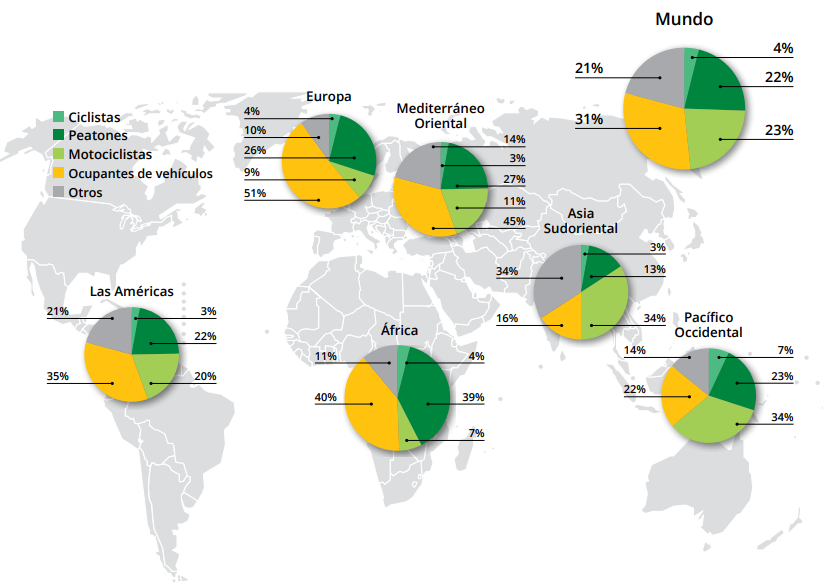
\includegraphics[width=0.9\textwidth, fbox]{imagenes/Cap1/oms1}
  \caption{Muertes por accidentes de tránsito por regi\'{o}n en función del tipo de usuario \protect\cite{Reference65}.}
  \label{fig:oms}  
  \end{center}
\end{figure}

Por otro lado seg\'{u}n la Unidad Operativa de Tr\'{a}nsito de Cochabamba los accidentes registrados en 2017 provocaron la muerte de 200 personas y dejaron aproximadamente 2200 heridos.
	
\vspace{5mm} %5mm vertical space

En la figura \ref{fig:arbol} se muestra las causas por las cuales se ocasiona un accidente de tr\'{a}nsito, se puede observar que gran parte de \'{e}stas se deben al factor humano sin embargo hay otras que conllevan factores medio-ambientales y mec\'{a}nicos, por lo que se hace imposible evitar completamente los mismos. 

\vspace{5mm} %5mm vertical space

Es por ello que se hace necesario el contar con mecanismos para prevenir y/o actuar de forma oportuna ante posibles accidentes de tr\'{a}nsito, motivo por el cual el presente trabajo se centra en estudiar los comportamientos de conducci\'{o}n, para as\'{i} generar alertas al encontrar un comportamiento an\'{o}malo en el manejo, de manera que se pueda evitar o en todo caso minimizar los efectos del mismo.

\begin{figure}[h!]
  \begin{center}	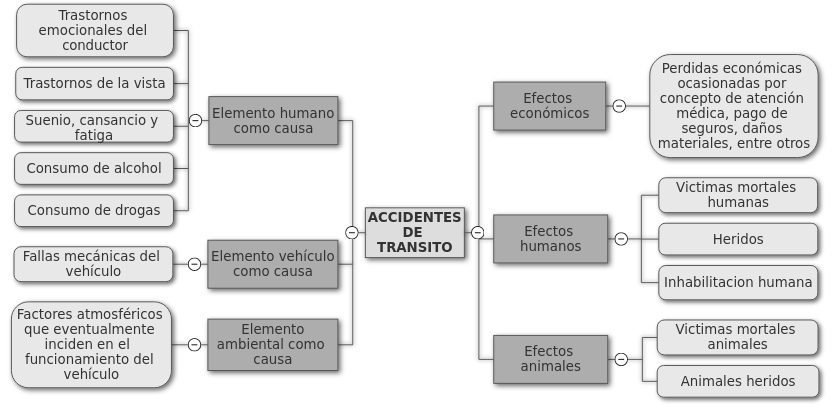
\includegraphics[width=1.0\textwidth, fbox]{imagenes/Cap1/arbol_p}
  \caption{\'{A}rbol de problemas (Elaboraci\'{o}n propia).}
  \label{fig:arbol}
  \end{center}
\end{figure}


\section{Objetivo general}

El objetivo general del presente trabajo es desarrollar un mecanismo de detecci\'{o}n de anomal\'{i}as de conducción, mediante el uso de un dispositivo móvil y algoritmos de Aprendizaje Automático, con el fin de alertar de forma oportuna el hallazgo de un patrón anómalo en el manejo, tal como cansancio, ebriedad, o problemas de salud, ej, epilepsia.

\section{Objetivos específicos}
\begin{itemize}

\item Capturar los parámetros de manejo de un conductor mediante el uso de sensores de un dispositivo móvil.
\item Escalar los parámetros de manejo mediante técnicas de pre-procesamiento de datos.
\item Generar un modelo de aprendizaje automático que se ajuste a un comportamiento normal de manejo.
\item Definir un método de detección de anomalías para generar una alerta de conducción anormal.
\item Evaluar el método de detección de anomalías con nuevas muestras.

\end{itemize}


\section{Justificación}

Los accidentes de tránsito cobran un número inaceptable de víctimas cada a\~{n}o, especialmente en las regiones m\'{a}s pobres del mundo. Esto se debe a diversos aspectos, pero el principal recae en el bajo nivel de conciencia ciudadana que existe, lo que conlleva a que muchas personas conduzcan bajo los efectos del alcohol, con exceso de velocidad, manipulando sus dispositivos m\'{o}viles, entre otros. Por ello este trabajo busca establecer patrones de comportamientos de conducci\'{o}n mediante el uso de un dispositivo m\'{o}vil y t\'{e}cnicas de Aprendizaje Autom\'{a}tico, de manera que se logre realizar una detecci\'{o}n de anomal\'{i}as de conducci\'{o}n oportuna.

\subsection{Justificaci\'{o}n pr\'{a}ctica}

Detectar anomal\'{i}as de conducci\'{o}n permite generar una alerta oportuna a las autoridades o a los agentes para que logren corregir sus conductas de conducci\'{o}n de forma r\'{a}pida. De esta manera se podr\'{a} evitar accidentes de tr\'{a}nsito o minimizar sus efectos, permitiendo as\'{i} reducir la cantidad de da\~{n}os, tanto materiales como personales.

\subsection{Justificaci\'{o}n metodol\'{o}gica}

El estudio realizado en el desarrollo del presente trabajo de investigaci\'{o}n permite resaltar la eficiencia de las t\'{e}cnicas de Inteligencia Artificial en la detecci\'{o}n de anomal\'{i}as.

\section{L\'{i}mites y alcances}

Debido a que la realizaci\'{o}n de pruebas de campo para \'{e}sta investigaci\'{o}n es bastante peligrosa, se limit\'{o} los ejemplos de conducci\'{o}n an\'{o}mala a:

\begin{itemize}
\item Frenos en seco.
\item Giros hacia la derecha e izquierda a alta velocidad.
\item Giros en zig zag bruscos.
\end{itemize}

\vspace{5mm} %5mm vertical space

Siendo as\'{i}, los experimentos y pruebas se realizaron s\'{o}lo sobre un peque\~{n}o conjunto de ejemplos an\'{o}malos, por lo tanto no se espera que el modelo de detecci\'{o}n propuesto funcione de manera correcta sobre aquellos ejemplos que no fueron considerados.

\section{M\'{e}todo de investigaci\'{o}n}

El presente estudio se realiz\'{o} con un enfoque experimental, teniendo como hip\'{o}tesis la siguiente:


\begin{center}
\textit{\large{¿Es posible detectar anomal\'{i}as de conducci\'{o}n mediante el uso de un dispositivo móvil y algoritmos de Aprendizaje Autom\'{a}tico?}}
\end{center}

